\subsection{Seitenwechsel}

\begin{figure}[H]
\centering
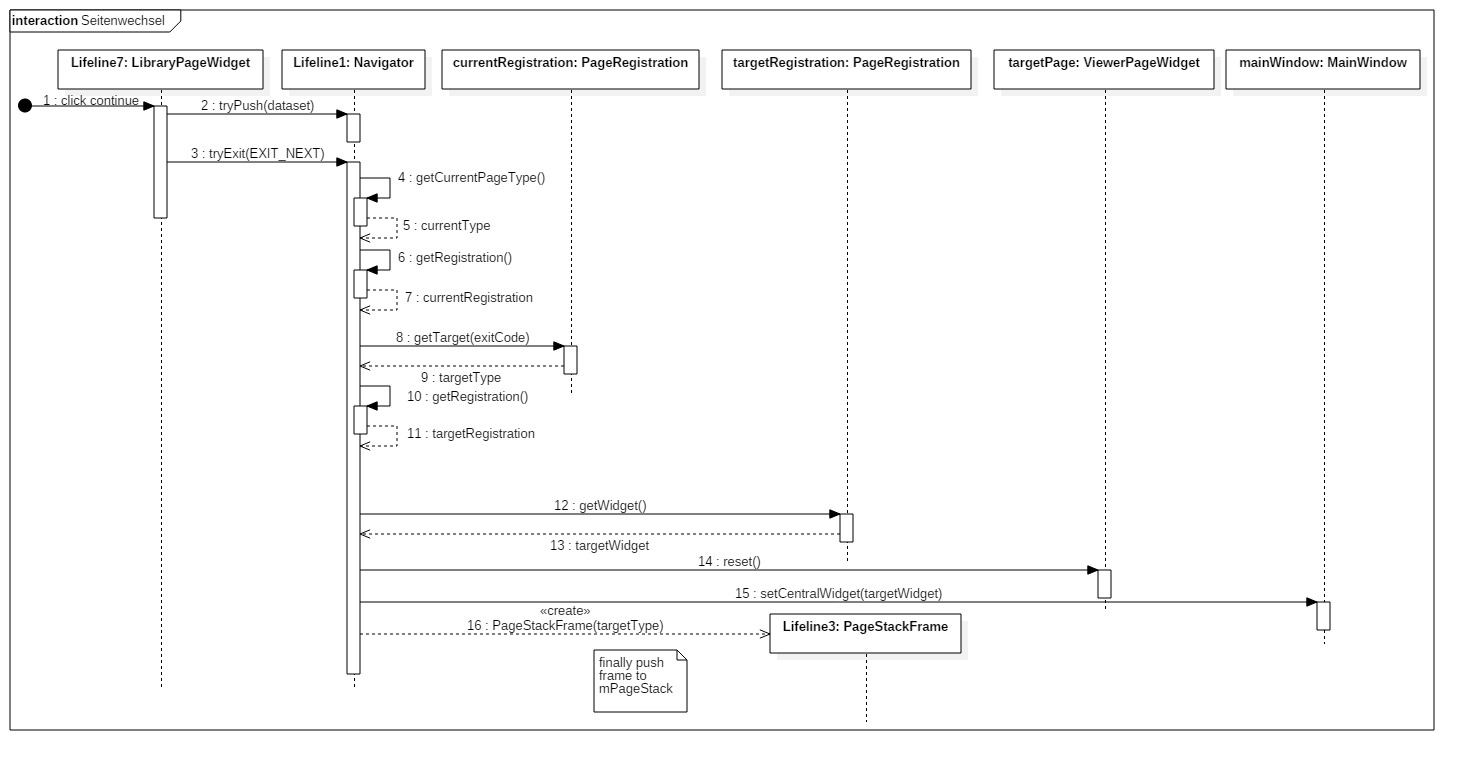
\includegraphics[width=\linewidth]{img/Sequenzdiagramme/Seitenwechsel}
\label{fig:seitenwechsel}
\end{figure}

Dieses Sequenzdiagramm beschreibt die Abläufe beim Seitenwechsel. Es wird der Übergang vom LibraryPageWidget zum ViewerPageWidget dargestellt. Das LibraryPageWidget übergibt dem Navigator über die Signal-Slot Verbindung den Pfad zum ausgewählten Datensatz. Der Navigator registriert das ViewerPageWidget als das PageWidget, das danach angezeigt werden soll. Danach erhält das MainWindow das ViewerPageWidget, um es anzuzeigen.

\pagebreak

\subsection{Suche starten}

\begin{figure}[H]
\centering
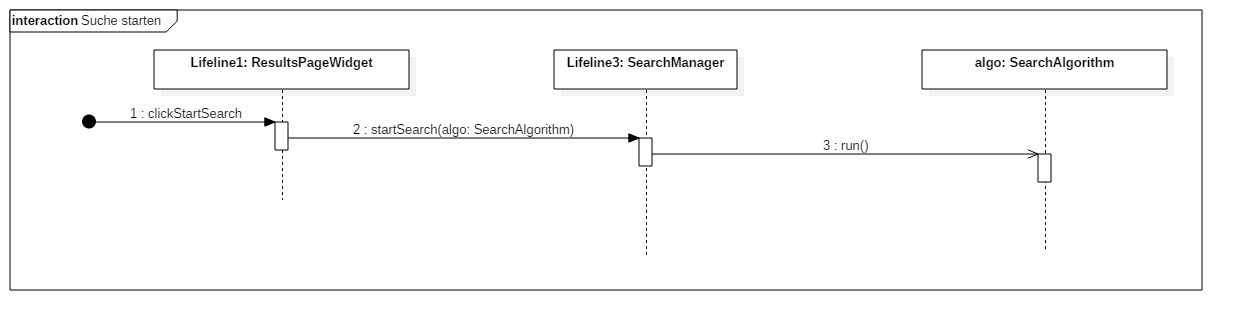
\includegraphics[width=\linewidth]{img/Sequenzdiagramme/SucheStarten}
\label{fig:sucheStarten}
\end{figure}
Nachdem der Benutzer den Button zum Start der Suche geklickt hat, übergibt das aktuelle PageWidget den Algorithmus an den SearchManager. Dieser startet die Suche.

\subsection{Suche terminieren}

\begin{figure}[H]
\centering
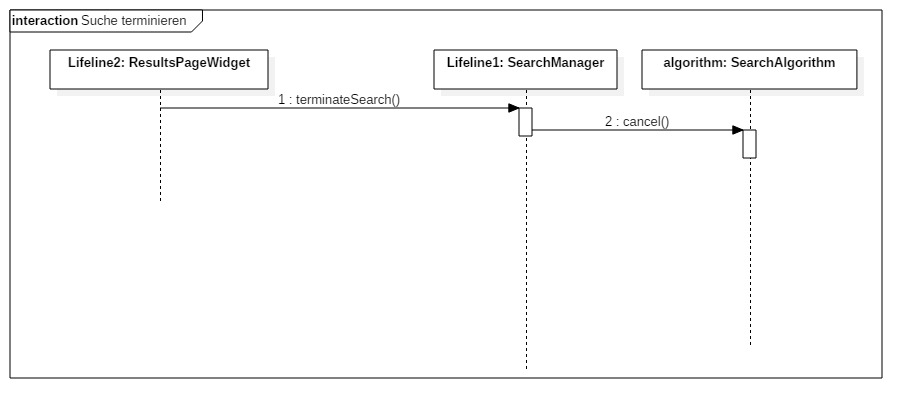
\includegraphics[width=\linewidth]{img/Sequenzdiagramme/SucheTerminieren}
\label{fig:sucheTerminieren}
\end{figure}
Das ResultsPageWidget veranlasst den SearchManager dazu, den Algorithmus zu beenden.

\subsection{Suchergebnis speichern}

\begin{figure}[H]
\centering
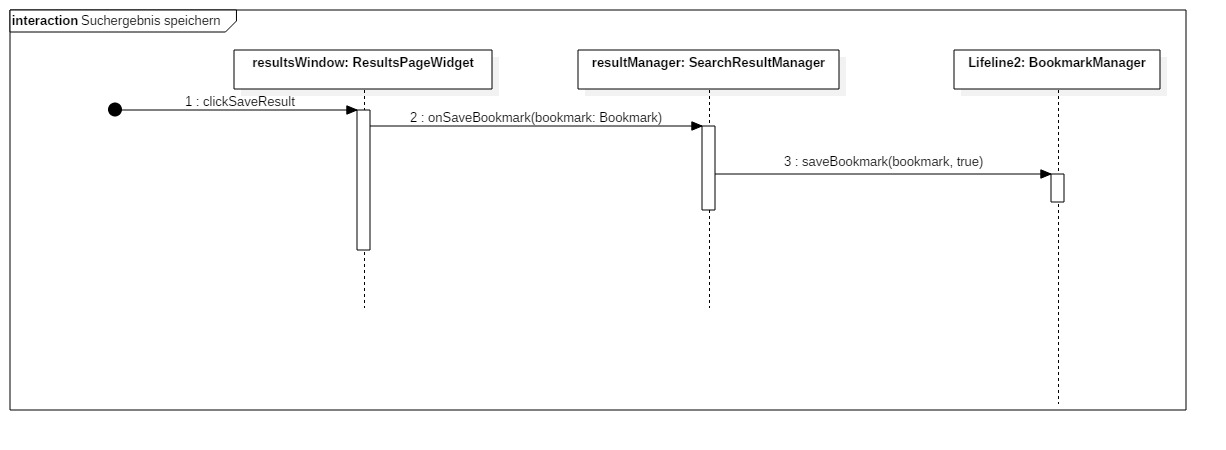
\includegraphics[width=\linewidth]{img/Sequenzdiagramme/SuchergebnisSpeichern}
\label{fig:suchergebnisSpeichern}
\end{figure}
Nachdem der Benutzer den Button zum Speichern des Suchergebnisses geklickt hat, übergibt das ResultsPageWidget dem SearchResultManager das Bookmark. Dieser ruft den BookmarkMangager zum Speichern auf.